%%%%%%%%%%%%%%%%%%%%%%%%%%%%%%%%%%%%%%%%%
% Arsclassica Article
% LaTeX Template
% Version 1.1 (1/8/17)
%
% This template has been downloaded from:
% http://www.LaTeXTemplates.com
%
% Original author:
% Lorenzo Pantieri (http://www.lorenzopantieri.net) with extensive modifications by:
% Vel (vel@latextemplates.com)
%
% License:
% CC BY-NC-SA 3.0 (http://creativecommons.org/licenses/by-nc-sa/3.0/)
%
%%%%%%%%%%%%%%%%%%%%%%%%%%%%%%%%%%%%%%%%%

%----------------------------------------------------------------------------------------
%	PACKAGES AND OTHER DOCUMENT CONFIGURATIONS
%----------------------------------------------------------------------------------------

\documentclass[
10pt, % Main document font size
a4paper, % Paper type, use 'letterpaper' for US Letter paper
oneside, % One page layout (no page indentation)
%twoside, % Two page layout (page indentation for binding and different headers)
headinclude,footinclude, % Extra spacing for the header and footer
BCOR5mm, % Binding correction
]{scrartcl}

%%%%%%%%%%%%%%%%%%%%%%%%%%%%%%%%%%%%%%%%%
% Arsclassica Article
% Structure Specification File
%
% This file has been downloaded from:
% http://www.LaTeXTemplates.com
%
% Original author:
% Lorenzo Pantieri (http://www.lorenzopantieri.net) with extensive modifications by:
% Vel (vel@latextemplates.com)
%
% License:
% CC BY-NC-SA 3.0 (http://creativecommons.org/licenses/by-nc-sa/3.0/)
%
%%%%%%%%%%%%%%%%%%%%%%%%%%%%%%%%%%%%%%%%%

%----------------------------------------------------------------------------------------
%	REQUIRED PACKAGES
%----------------------------------------------------------------------------------------

\usepackage[
nochapters, % Turn off chapters since this is an article        
beramono, % Use the Bera Mono font for monospaced text (\texttt)
eulermath,% Use the Euler font for mathematics
pdfspacing, % Makes use of pdftex’ letter spacing capabilities via the microtype package
dottedtoc, % Dotted lines leading to the page numbers in the table of contents
]{classicthesis} % The layout is based on the Classic Thesis style


\usepackage{arsclassica} % Modifies the Classic Thesis package
\usepackage[left=0.5in, right=0.5in]{geometry}

\usepackage[T1]{fontenc} % Use 8-bit encoding that has 256 glyphs

\usepackage[utf8]{inputenc} % Required for including letters with accents

\usepackage{graphicx} % Required for including images
\graphicspath{{Figures/}} % Set the default folder for images

\usepackage{enumitem} % Required for manipulating the whitespace between and within lists

\usepackage{lipsum} % Used for inserting dummy 'Lorem ipsum' text into the template

\usepackage{subfig} % Required for creating figures with multiple parts (subfigures)

\usepackage{amsmath,amssymb,amsthm} % For including math equations, theorems, symbols, etc

\usepackage{varioref} % More descriptive referencing

\usepackage{color}

%----------------------------------------------------------------------------------------
%	THEOREM STYLES
%---------------------------------------------------------------------------------------

\theoremstyle{definition} % Define theorem styles here based on the definition style (used for definitions and examples)
\newtheorem{definition}{Definition}

\theoremstyle{plain} % Define theorem styles here based on the plain style (used for theorems, lemmas, propositions)
\newtheorem{theorem}{Theorem}

\theoremstyle{remark} % Define theorem styles here based on the remark style (used for remarks and notes)

%----------------------------------------------------------------------------------------
%	HYPERLINKS
%---------------------------------------------------------------------------------------

\hypersetup{
%draft, % Uncomment to remove all links (useful for printing in black and white)
colorlinks=true, breaklinks=true, bookmarks=true,bookmarksnumbered,
urlcolor=webbrown, linkcolor=RoyalBlue, citecolor=webgreen, % Link colors
pdftitle={}, % PDF title
pdfauthor={\textcopyright}, % PDF Author
pdfsubject={}, % PDF Subject
pdfkeywords={}, % PDF Keywords
pdfcreator={pdfLaTeX}, % PDF Creator
pdfproducer={LaTeX with hyperref and ClassicThesis} % PDF producer
} % Include the structure.tex file which specified the document structure and layout

\hyphenation{Fortran hy-phen-ation} % Specify custom hyphenation points in words with dashes where you would like hyphenation to occur, or alternatively, don't put any dashes in a word to stop hyphenation altogether

%----------------------------------------------------------------------------------------
%	TITLE AND AUTHOR(S)
%----------------------------------------------------------------------------------------

\title{\normalfont\spacedallcaps{AC6 Curtain Distribution Running Report}} % The article title

%\subtitle{Subtitle} % Uncomment to display a subtitle

\author{\spacedlowsmallcaps{Mykhaylo Shumko}} 


%\date{} % An optional date to appear under the author(s)

%----------------------------------------------------------------------------------------

\begin{document}


%----------------------------------------------------------------------------------------
%	HEADERS
%----------------------------------------------------------------------------------------

\renewcommand{\sectionmark}[1]{\markright{\spacedlowsmallcaps{#1}}} % The header for all pages (oneside) or for even pages (twoside)
%\renewcommand{\subsectionmark}[1]{\markright{\thesubsection~#1}} % Uncomment when using the twoside option - this modifies the header on odd pages
\lehead{\mbox{\llap{\small\thepage\kern1em\color{halfgray} \vline}\color{halfgray}\hspace{0.5em}\rightmark\hfil}} % The header style

\pagestyle{scrheadings} % Enable the headers specified in this block

%----------------------------------------------------------------------------------------
%	TABLE OF CONTENTS & LISTS OF FIGURES AND TABLES
%----------------------------------------------------------------------------------------

\maketitle % Print the title/author/date block

\setcounter{tocdepth}{2} % Set the depth of the table of contents to show sections and subsections only

\tableofcontents % Print the table of contents

\listoffigures % Print the list of figures

\listoftables % Print the list of tables

%----------------------------------------------------------------------------------------
%	INTRODUCTION
%----------------------------------------------------------------------------------------

\section{Introduction}
This project aims to quantify the statistical properties of curtains, and test the hypothesis proposed by Bern that curtains are microburst remnants in the drift loss cone (DLC).

\section{Curtain Selection}
These curtains were selected using Paul's burst parameter with a threshold of 5. Transmitter noise was removed with the procedure described in the AC6 microburst distribution paper. Times when the burst parameter value was above the threshold, and a inter-spacecraft spatial correlation $> 0.8$ are curtain candidates. I inspected each candidate curtain and removed the noisy and ambiguous detections. In the end, 933 curtains were confirmed, and I have about 100 example curtain plots that I've saved. A few examples of curtains are shown in Fig. \ref{curtain_examples}. In all of these cases, AC6A (i.e. not AC6B) was ahead by the annotated in-track lag. The reason for the mixup is when I started going through the candidate detections I was not certain what AC6 unit was ahead. Paul confirmed that In-track lag $ > 0$ means AC6A is ahead.


\begin{figure}[htb]
\centering
\subfloat[AC6A ahead by 22 s]{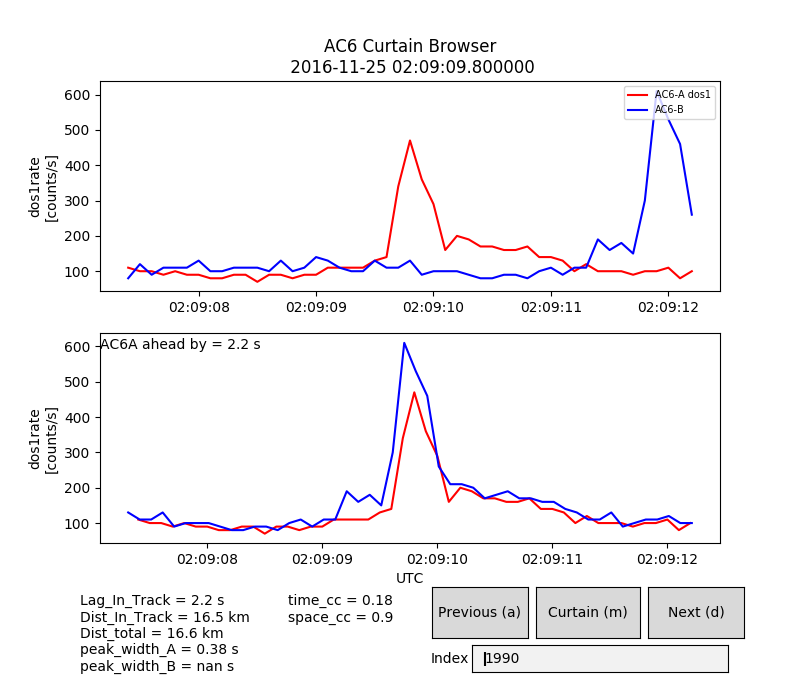
\includegraphics[width=.45\columnwidth]{20161125_0209_2s_curtain.png}} \quad
\subfloat[AC6A ahead by 8 s]{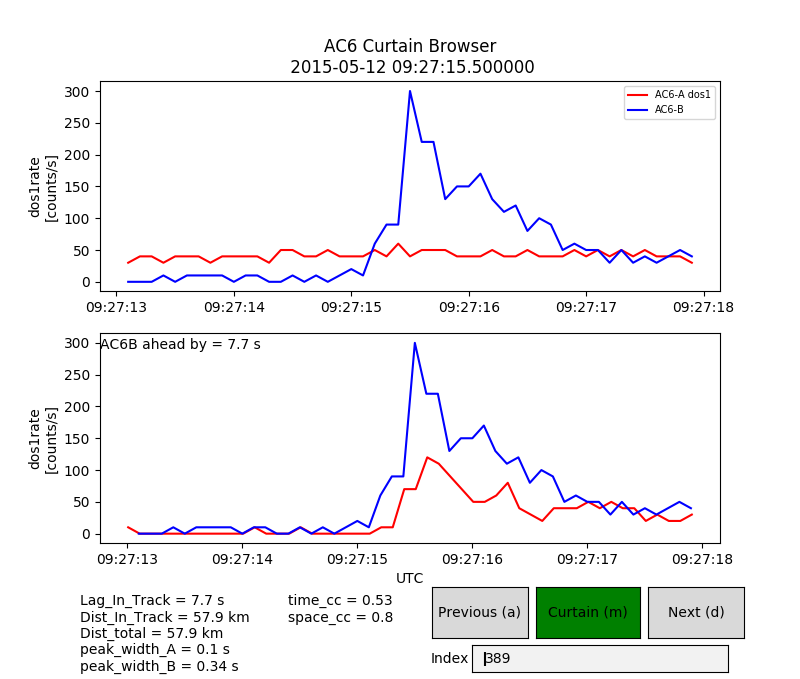
\includegraphics[width=.45\columnwidth]{20150512_8s_curtain.png}\label{fig:ipsum}} \\
\subfloat[AC6A ahead by 7 s]{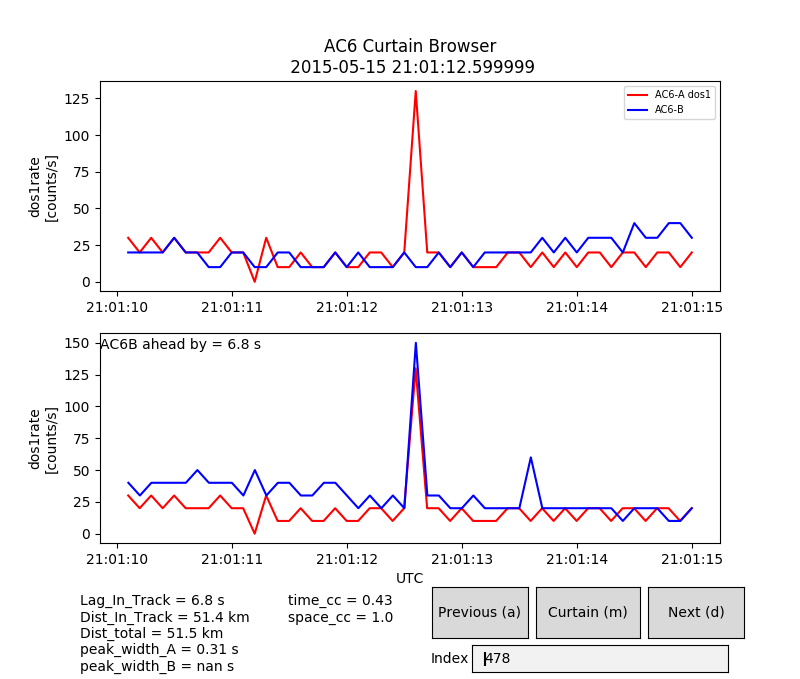
\includegraphics[width=.45\columnwidth]{20150515_7s_curtain.png}} \quad
\subfloat[AC6A ahead by 4 s]{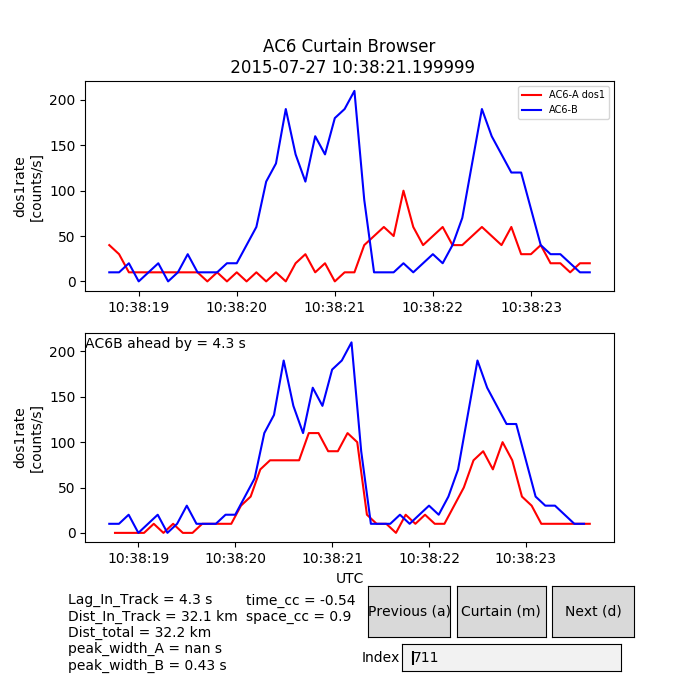
\includegraphics[width=.45\columnwidth]{20150727_1038_4s_curtain.png}}
\caption[Curtain examples]{Four examples of curtains observed by AC6. The pair of plots in each subplot shows the time-aligned dos1 count rates in the top plot, and the shifted time series in the bottom plot contrasts what AC6 observed over the same spatial location. The low correlation at the same time and high correlation at the same spatial location implies that these microburst-like features are curtains. NOTE: The plot annotations (not subplot caption!) are not correct regarding to what AC6 unit was ahead. The subplot caption is correct.}
\label{curtain_examples}
\end{figure}

\section{Global Statistics of Curtains}

\subsection{L-MLT distributions}
Figures \ref{unnormalized_dist} and \ref{normalized_dist} show the distributions of curtains in L and MLT. Figure \ref{unnormalized_dist}a shows the unnormalized number of curtains observed in each L-MLT bin. Curtains were observed in the late morning sector, and in the late evening sectors. The AC6 orbit did not sample much in the 3-6 MLT, and 14-18 MLT regions as shown in Fig. \ref{unnormalized_dist}b, so in reality curtains probably occur in all MLTs.

Since Fig. \ref{unnormalized_dist}b shows that the AC6 orbit was highly preferential in MLT, this bias needs to be accounted for and the number of curtains normalized. Figure \ref{normalized_dist}a shows the normalized distribution of curtains. With the normalization, it looks like the late dawn and evening curtains occur at similar rates, although the slim number of 10 Hz samples at higher L shells and at late MLTs means that the normalized number of curtains there may be nonphysical.

\begin{figure}
\centering
\includegraphics[width=0.9\paperwidth]{curtain_dist_norm_false.png}
\caption{Equatorial distribution of curtains. Panel a shows the unnormalized distribution of curtains in L-MLT. Panel b shows the number of quality 10 Hz samples taken at the same position.}
\label{unnormalized_dist}
\end{figure}

\begin{figure}
\centering
\includegraphics[width=0.9\paperwidth]{curtain_dist_norm_true.png}
\caption{Same as Fig. \ref{unnormalized_dist}, but normalized.}
\label{normalized_dist}
\end{figure}

\subsection{Curtains in the Bounce Loss Cone (BLC)}
Particles that impact the atmosphere are lost during that bounce motion. We found curtains in the bounce loss cone, a region in the North Atlantic near and above Iceland.

The bounce loss cone is magnetically connected to the SAA, where Earth's magnetic field is weakest near Earth's surface. A particle observed in the BLC in the northern hemisphere will descend below 100 km altitude. At these altitudes the particle has a high chance of scattering with the atmosphere and be lost from the magnetosphere. 

We found multiple curtain elections that, when given the chance to execute their cyclical bounce motion, will descend below Earth's surface in the SAA. An election can not survive that trip. We observed curtains for $4-8$ AC6 in-track separations, longer than the $1-2$ second 35 keV electron bounce period.

\subsection{Integrated curtain count comparison between the leading and following AC6 unit}

For the 0.5 s integration, 280 curtains had more leader counts and the remaining 653 had higher follower counts. \\

\noindent For the 1 s integration, 272 curtains had more leader counts and the remaining 661 had higher follower counts.

With Paul's baseline subtraction - 10th percentile over a 30 s interval - no substatial changes are noticed.

Tighting up the ratio of the pitch angles (PA) reduces the scatter about the diagonal, but the mean ratio is still too close to 1.

\iffalse
\begin{figure}[htb]
\centering
\subfloat[AC6A ahead by 22 s]{\includegraphics[width=.45\columnwidth]{curtain_leader_follower_counts_05_integration_bkg_false.png}} \quad
\subfloat[AC6A ahead by 8 s]{\includegraphics[width=.45\columnwidth]{curtain_leader_follower_counts_10_integration_bkg_false.png}\label{fig:ipsum}}
\caption{Leader-follower count rate comparison without background subtraction and integrating over 0.5 seconds on the left panel, and 1 second on the right panel.}
\label{curtain_examples}
\end{figure}
\fi

\begin{figure}[ht]
\centering
\includegraphics[width=0.9\paperwidth]{curtain_leader_follower_counts_05_integration_bkg_false_3.png}
\caption{Leader-follower count rate comparison without background subtraction and integrating over 0.5 seconds.}
\label{curtain_leader_follower_05}
\end{figure}

\begin{figure}[ht]
\centering
\includegraphics[width=0.9\paperwidth]{curtain_leader_follower_counts_10_integration_bkg_false_3.png}
\caption{Same format as \ref{curtain_leader_follower_05} except the integration time is 1 second.}
\label{curtain_leader_follower_10}
\end{figure}

\section{Path Forward}
\begin{enumerate}
\item Add a filter to not normalize the curtains in the under-sampled L-MLT bins e.g. less than 10 curtains were observed or less than 1000 10 Hz samples were gathered in that L-MLT bin.
\item Compare the curtain and microburst distributions.
\item Look at curtain occurrence rates as a function of MLT and longitude (local time)
\item Calculate the integrated counts for each curtain over 0.5 and 1 s intervals. Make scatter plot of leading spacecraft integrated counts on the x-axis and trailing spacecraft counts on the y-axis. If Bern's hypothesis is true, there should be lots of observations in the upper-left corner, and not many near the diagonal.
\item Cross-calibrate the AC6 units by calculating average counts during every pass they took data together.
\item Check $\alpha$ when curtains were observed. By looking at the README and the AC6 configuration, the pitch angles should be similar. Bern's paper mentions that the AC6 dos1 count rates are cross-calibrated within a factor of two.

 
\end{enumerate}

%----------------------------------------------------------------------------------------
%	BIBLIOGRAPHY
%----------------------------------------------------------------------------------------

%\renewcommand{\refname}{\spacedlowsmallcaps{References}} % For modifying the bibliography heading

%\bibliographystyle{unsrt}

%\bibliography{sample.bib} % The file containing the bibliography

%----------------------------------------------------------------------------------------

\end{document}